%; whizzy paragraph -pdf xpdf -latex ./whizzypdfptex.sh
%; whizzy-paragraph "^\\\\begin{frame}\\|\\\\emtext"
% latex beamer presentation.
% platex, latex-beamer $B$G%3%s%Q%$%k$9$k$3$H$rA[Dj!#(B 

%     Tokyo Debian Meeting resources
%     Copyright (C) 2012 Junichi Uekawa
%     Copyright (C) 2012 Nobuhiro Iwamatsu

%     This program is free software; you can redistribute it and/or modify
%     it under the terms of the GNU General Public License as published by
%     the Free Software Foundation; either version 2 of the License, or
%     (at your option) any later version.

%     This program is distributed in the hope that it will be useful,
%     but WITHOUT ANY WARRANTY; without even the implied warreanty of
%     MERCHANTABILITY or FITNESS FOR A PARTICULAR PURPOSE.  See the
%     GNU General Public License for more details.

%     You should have received a copy of the GNU General Public License
%     along with this program; if not, write to the Free Software
%     Foundation, Inc., 51 Franklin St, Fifth Floor, Boston, MA  02110-1301 USA

\documentclass[cjk,dvipdfmx,12pt]{beamer}
\usetheme{Tokyo}
\usepackage{monthlypresentation}

%  preview (shell-command (concat "evince " (replace-regexp-in-string "tex$" "pdf"(buffer-file-name)) "&")) 
%  presentation (shell-command (concat "xpdf -fullscreen " (replace-regexp-in-string "tex$" "pdf"(buffer-file-name)) "&"))
%  presentation (shell-command (concat "evince " (replace-regexp-in-string "tex$" "pdf"(buffer-file-name)) "&"))

%http://www.naney.org/diki/dk/hyperref.html
%$BF|K\8l(BEUC$B7O4D6-$N;~(B
\AtBeginDvi{\special{pdf:tounicode EUC-UCS2}}
%$B%7%U%H(BJIS$B7O4D6-$N;~(B
%\AtBeginDvi{\special{pdf:tounicode 90ms-RKSJ-UCS2}}

\title{$BEl5~%(%j%"(BDebian$BJY6/2q(B}
\subtitle{systemd}
\author{$B4d>>(B $B?.MN(B\\iwamatsu@debian.org}
\date{2012$BG/(B11$B7n(B17$BF|(B}
\logo{
\includegraphics[width=8cm]{image200607/openlogo-light.eps}}

\begin{document}

\frame{\titlepage{}}

%\begin{frame}[containsverbatim]
%
%$B$*$^$($i!"$A$g$C$H(B $B!V(B\texttt{ps ax | grep systemd}$B!W(B $B<B9T$7$F$_$m!*(B
%\begin{commandline}
%
%hooo%
%
%\end{commandline}
%\end{frame}

\begin{frame}{$B$O$8$a$K(B}

\begin{itemize}
\item $B@$$NCf$N<gMW$J(BLinux$B%G%#%9%H%j%S%e!<%7%g%s$O(B 
SysVinit $B$N(B init scripts $B$+$iB>$N(Binit $B%7%9%F%`$K0\9T$7$D$D$"$k!J$O$:!K!#(B
\item Fedora$B$d(BArch Linux$B$,(Bsystemd $B$K0\9T$r;O$a$?$H$$$&$3$H$b$"$j!"(B
$B0lIt$G@9$j>e$,$C$F$$$k!J0$I!6+4-$H$b$$$&!K!#(B
\item $B$^$5$+(B $B$$$^$@$K(B SysVinit $B$r;H$C$F$J$$$h$M!)(B
\item Debian$B$H(Bsystemd$B$K$D$$$F$^$H$a$?!#(B
\end{itemize}

\end{frame}

\begin{frame}{systemd$B$H$O!)(B}

\begin{itemize}
\item RedHat $B$K6P$a$F$$$k(B Lennart Poettering $B;a$K$h$C$F3+H/$5$l$F$$$k!#(B
\item init $B$NBeBX%W%m%0%i%`!#(B
\item $B<B:]$K$O(B init $B$NBeBX$@$1$G$O$J$/!"(BLinux $B$N%5!<%S%9!J%G!<%b%s!K4IM}%U%l!<%`%o!<%/!#(B
%Linux $B%+!<%M%kMQ$N%G%P%$%94IM}%D!<%k$G$"$k(B udev $B$,(B systemd $B$N%=!<%9$K%^!<%8(B
%$B$5$l$F$$$^$9!#%m%0%7%9%F%`$b$"$k!#>-Mh$O(B cron $B$d(B acpid $B$J$I$NBeBX$(5!G=$r(B
%$BDs6!$9$kM=Dj$i$7$$!#(B
\item $B:#$^$G$N(Binit$B%7%9%F%`$N0c$$(B
  \begin{itemize}
  \item $B%5!<%S%9$N%W%m%;%94IM}$r(B pid $B$G$O$J$/!"(Bcgroups $B$r;H$&!#(B
  \item $B%5!<%S%9$N5/F0$r%=%1%C%H$H%P%9(B(dbus)$B$r;H$&!#(B
  \item $B%5!<%S%9$N0MB84X78$,$"$j!"$3$l$K$h$C$F%7%9%F%`N)$A>e$2=hM}$r$h$jJBNsE*$K9T$($k!#(B
  \item System V $B%9%?%$%k$H(BBSD$B%9%?%$%k$NN>J}$r%5%]!<%H$7$F$$$k!#(B
  \item CosoleKit $B$H$NO"7H!#(B
  \end{itemize}
\end{itemize}

\end{frame}


\begin{frame}
\includegraphics[width=1\hsize]{image201211/systemd-relation.eps}
\end{frame}

\begin{frame}{systemd$B$H$O!)(B}

\begin{itemize}
\item $B3+H/$O(B freedesktop.org$B$G9T$o$l$F$*$j!"3+H/$O3hH/$G=5$K0lEY$O%P!<%8%g%s%"%C%W!#(B
\item $B:G?7%P!<%8%g%s$O(B v195$B!#(B
\item \url{http://cgit.freedesktop.org/systemd/systemd/}
\end{itemize}

\end{frame}

\begin{frame}{SysVinit $B$HHf$Y$?(B systemd $B$NMxE@(B}

\begin{itemize}
\item $B@_Dj$,MF0W!#(B
\item $B5/F0$,Aa$$!#(B
\item $B%+!<%M%k%b%8%e!<%k$NA`:n!"%;%C%7%g%s4IM}!"%m%04IM}!"%G%#%9%/$N0E9f2=$J$I$,E}9g$5$l$F$$$k!#(B
\end{itemize}

$B$=$NB>!"3+H/<T$K$h$k@bL@$,(B\url{http://0pointer.de/blog/projects/why.html}
$B$K$"$k!#(B

\end{frame}

\begin{frame}{SysVinit $B$HHf$Y$?(B systemd $B$N7gE@(B/$BIT0B(B}

\begin{itemize}
\item $B$"$i$f$k4pK\%5!<%S%9(B(cron$B$J$I$b(B)$B$r$^$H$a$k$H$$$&ATBg$JJ*8l!#(B
\item $BF|K\8l%I%-%e%a%s%H$,$J$$!"$0$i$$!)(B
\item kFreeBSD $B$G$b4hD%$l$P$&$4$/$i$7$$!#!J$I$&$d$C$F$k$N$+$OITL@!K(B
\end{itemize}

\end{frame}

\begin{frame}{Debian$B$G;H$&(B}

\begin{itemize}
\item systemd $B$O$b$A$m$s(B Debian $B$G$bDs6!$5$l$F$$$k(B
\item testing / unstable $B$G(B v44 $B$,MxMQ$G$-$k(B\\
$B:G?7HG$H%P!<%8%g%s$K:9$,$"$k$,!"%"%C%W%9%H%j!<%`$G(B
$BIQHK$K%P!<%8%g%s%"%C%W$9$k$N$G%P!<%8%g%s$O$"$^$jLdBj$G$O$J$$(B
v44 $B$G$b(B systemd $B$r==J,$K;H$&$3$H$,$G$-$k(B

\item $B$$$^$N$H$3$m(B Debian$B$K4X$9$k>pJs$O(B \url{http://wiki.debian.org/systemd}
$B$K$^$H$^$C$F$$$k$,>pJs$,>/$J$/!"FbMF$b8E$$(B
\end{itemize}

\end{frame}

\begin{frame}[containsverbatim]{$B%$%s%9%H!<%k(B}

\begin{itemize}
\item apt-get / aptitude $B$G%$%s%9%H!<%k$G$-$k!#(B
\item Linux $B%+!<%M%k$O(B 2.6.39 $B0J>e!"(Bdevtmpfs, fanotify, autofs4, cgroups $B$,M-8z$K$J$C$F$$$kI,MW$,$"$k!#(B
\end{itemize}

\end{frame}

\begin{frame}[containsverbatim]{$B%$%s%9%H!<%k(B}

$B%$%s%9%H!<%k$O0J2<$N$h$&$K<B9T$9$k!#(B

\begin{commandline}
$ sudo apt-get install systemd
\end{commandline}
%$

$B0J2<$N%Q%C%1!<%8$,0MB84X78$G%$%s%9%H!<%k$5$l$k!#(B
\begin{commandline}
libsystemd-daemon0
libsystemd-id128-0
libsystemd-journal0
libpam-systemd
\end{commandline}
%$

\end{frame}

\begin{frame}[containsverbatim]{$B%$%s%9%H!<%k(B}

\begin{itemize}
\item $B<!$K%V!<%H%m!<%@$K(Binit$B;XDj$rDI2C$9$k(B
\item GRUB $B$r;H$C$F$$$k>l9g!"(B\texttt{/etc/default/grub} $B$N(B
\texttt{GRUB\_CMDLINE\_LINUX\_DEFAULT} $B$K(B {\bf init=/lib/systemd/systemd} $B$rDI5-$9$k(B
 
\begin{commandline}
$BJQ99A0(B:
GRUB_CMDLINE_LINUX_DEFAULT="quiet"
$BJQ998e(B:
GRUB_CMDLINE_LINUX_DEFAULT="quiet init=/lib/systemd/systemd"
\end{commandline} 
%$

\end{itemize}

\end{frame}

\begin{frame}[containsverbatim]{$B%$%s%9%H!<%k(B}

\begin{itemize}
\item $BJQ998e!"(B{\bf update-grub}$B$r<B9T$7!"(BGRUB $B$K@_Dj$rH?1G$9$k!#(B
\item $B$=$7$F%j%V!<%H$9$k!#(B
\item $B@_Dj$,4V0c$C$F$$$J$$$1$l$P(B systemd $B$GN)$A>e$,$k$O$:!#(B
\end{itemize}

\begin{commandline}
$ sudo update-grub
.....
$ sudo reboot 
\end{commandline}
%$

\end{frame}

\begin{frame}[containsverbatim]{$B5/F0B.EY(B}

\begin{itemize}
\item systemd $B$O%"%J%i%$%6$r%G%U%)%k%H$G%5%]!<%H$7$F$$$k!#(B\\
SysVinit $B$@$H(B bootchart2 $B$GB,Dj$9$kI,MW$,$"$k!#(B
\item $B5/F0$K$+$+$C$?;~4V$r3NG'$9$k$K$O(B \texttt{systemd-analyze} $B$r<B9T$9$k!#(B
\begin{commandline}
$ systemd-analyze 
Startup finished in 1831ms (kernel) + \ 
     5669ms (userspace) = 7500ms
\end{commandline}
%$
\end{itemize}
\end{frame}

\begin{frame}[containsverbatim]{$B5/F0B.EY(B}

\begin{itemize}

\item $B$^$?!"2hA|$G3NG'$7$?$$>l9g$K$O(B \texttt{prop} $B%*%W%7%g%s$r;XDj$7$F<B9T$9$k!#(B\\
  SVG $B%U%)!<%^%C%H$G=PNO$5$l$k$N$G!"%j%@%$%l%/%H$7$F%U%!%$%k$KJ]B8$9$k!#(B
\begin{commandline}
$ systemd-analyze plot > systemd-boot.svg
\end{commandline}
%$
\end{itemize}

\end{frame}

\begin{frame}

\begin{center}
\includegraphics[width=1\hsize]{image201211/systemd-boot.eps}
\end{center}
\end{frame}

\begin{frame}[containsverbatim]{$B5/F0B.EY(B}

$B;n$7$K<+J,$,>oMQ$7$F$$$k4D6-$G5/F0;~4V$rB,Dj$7$?$H$3$m!"(B
SysVinit $B$OLs(B15$BIC!"(Bsystemd $B$OLs(B10$BIC$@$C$?!#(B 

\end{frame}

\begin{frame}{$BMQ8l(B}

systemd $B$r07$&$K$O@lLgMQ8l$,=P$F$/$k$N$G@bL@$9$k!#(B

\end{frame}

\begin{frame}{$B%f%K%C%H(B}

\begin{itemize}
\item systemd $B$G$O%G!<%b%s$J$I$N@)8fBP>]$N$3$H$r%f%K%C%H$H8F$V!#(B
\item $B%f%K%C%H$K$O%5!<%S%9!"%G%P%$%9!"%^%&%s%H%]%$%s%H$J$I!"$$$/$D$+$N<oN`$,$"$k!#(B
\item $B$3$N%f%K%C%H$O%F%-%9%H%U%!%$%k$G5-=R$5$l!"(B\texttt{/lib/systemd/system/} $B0J2<$K3JG<$5$l$F$$$k!#(B
\item $B3F%f%K%C%H$O3HD%;R$r;}$A!"%5!<%S%9$N>l9g$O(B\texttt{.service}$B$H$J$C$F$$$k!#(B
\end{itemize}

\end{frame}

\begin{frame}{$B%f%K%C%H(B}

\begin{table}[htb]
\begin{center}
  \begin{tabular}{ll}
    $B%f%K%C%H$N<oN`(B & $B@bL@(B \\
    service & $B%5!<%S%9(B \\
    socket & $B%=%1%C%H$G5/F0$9$k$?$a$N%=%1%C%HDj5A(B \\
    target & $B3F%5!<%S%9$rF14|$5$;$k$?$a$NDj5A(B \\
    device & udev $B$G4IM}$9$k%G%P%$%9(B \\
    snapshot & $B$"$k;~E@$N(Binit $B$N>uBV(B \\
    timer & $B%$%Y%s%H$+$i;~4V7P2a(B \\
    path & $B4F;k$9$k%Q%9(B \\
    mount & $B%^%&%s%H%]%$%s%H(B \\
    swap & $B%9%o%C%W(B \\
    automaount & $B<+F0%^%&%s%H%]%$%s%H(B \\
  \end{tabular}
%\caption{systemd $B$GDs6!$9$k%f%K%C%H(B}
%\label{tbl:unit}
\end{center}
\end{table}

mount, swap, automout $B$O5/F0;~$K(B \texttt{/etc/fstab} $B$+$i<+F0E*$K(B
$B%f%K%C%H$r@8@.$9$k!#(B

\end{frame}

\begin{frame}{$B%?!<%2%C%H(B}
\begin{itemize}
\item SysVinit $B$N(B runlevel $BAjEv$N$b$N!#(B
\item $B$3$l$O%G%#%9%H%j%S%e!<%7%g%s$K$h$C$F0[$J$k!#(B
\item Debian$B$N>l9g$O0J2<$NDL$j!#(B

\begin{table}[h]
\begin{center}
  \begin{tabular}{ll}
    run level & systemd $B$N%?!<%2%C%H(B \\
    0 & poweroff.target \\
    1 & rescue.target \\
    2 - 5 & multi-user.target \\
    6 & reboot.target \\
  \end{tabular}
%\caption{run level$B$H%?!<%2%C%H$NBP1~(B}
%\label{tbl:target}
\end{center}
\end{table}
\end{itemize}
\end{frame}

\begin{frame}{$B%?!<%2%C%H(B}

\begin{itemize}
\item $B$3$NB>$K(Bgraphical.target $B$H(B emergency.target $B$,$"$k!#(B
\item graphical.target X $B$K$h$k5/F0$r9T$&$H$-$K8F$P$l$k%?!<%2%C%H(B
\item emergency.target $B$O>c32$,5/$3$C$?;~$K5/F0$G$-$k$h$&$K$9$k$?$a$N%?!<%2%C%H!#(B
\item $B%?!<%2%C%H$O%+!<%M%k$N%V!<%H%*%W%7%g%s$K(B \texttt{systemd.unit=}$B$G;XDj$G$-$k!#(B
\item $B2?$b;XDj$7$J$$>l9g$O(Bdefault.target $B$,8F$P$l$k$h$&$K$J$C$F$$$k!#(B
\end{itemize}

\end{frame}

\begin{frame}{$B%f%K%C%H$NA`:nJ}K!(B}

\begin{itemize}
\item systemd $B$K0\9T$7$?8e!"%G!<%b%sEy$N@)8f$O(B /etc/init.d/ $B0J2<$r<B9T$9$k$N$G$O$J$/!"(B{\bf systemctl}
$B%3%^%s%I$r;H$C$FA`:n$9$k!#(B
\item $B0J2<$K%f%K%C%H$NA`:nJ}K!$K$D$$$F@bL@$9$k!#(B
\end{itemize}

\end{frame}

\begin{frame}[containsverbatim]{$B5/F0$7$F$$$k%f%K%C%H$rI=<($9$k(B}

$B5/F0$7$F$$$k%f%K%C%H$rI=<($9$k$K$O(B sytemctl $B$r<B9T$9$k!#(B

\begin{commandline}
$ systemctl
...
console-setup.service     loaded active exited        LSB: Set console font and 
cron.service              loaded active running       LSB: Regular background pr
dbus.service              loaded active running       D-Bus System Message Bus
debian-fixup.service      loaded active exited        Various fixups to make sys
exim4.service             loaded active running       LSB: exim Mail Transport A
getty@tty1.service        loaded active running       Getty on tty1
ifup@eth0.service         loaded active exited        ifup for eth0
...
\end{commandline}
%$

\end{frame}

\begin{frame}[containsverbatim]{$BA4$F$N%f%K%C%H$rI=<($9$k(B}

$BA`:n$G$-$k%f%K%C%H$rI=<($9$k$K$O(B \texttt{--all} $B$r;XDj$9$k!#(B
 
\begin{commandline}
$ systemctl --all
UNIT                      LOAD   ACTIVE   SUB       JOB DESCRIPTION
proc-sys...misc.automount loaded active   waiting       Arbitrary Executable Fil
dev-cdrom.device          loaded active   plugged       QEMU_DVD-ROM
dev-disk...QM00003.device loaded active   plugged       QEMU_DVD-ROM
dev-disk...QM00001.device loaded active   plugged       QEMU_HARDDISK
dev-disk...2dpart1.device loaded active   plugged       QEMU_HARDDISK
dev-disk...2dpart2.device loaded active   plugged       QEMU_HARDDISK
...
\end{commandline}
%$

\end{frame}

\begin{frame}[containsverbatim]{$B%f%K%C%H$N>uBV$r3NG'$9$k(B}

$B%f%K%C%H$N>uBV$r3NG'$9$k$K$O!"(B\texttt{status} $B%*%W%7%g%s$K3NG'$7$?$$%f%K%C%HL>$r(B
$B;XDj$7$F<B9T$9$k!#(B

$B0J2<$K(B rsyslog.service $B%f%K%C%H$N>uBV$r3NG'$9$kNc$r<($9!#(B
\begin{commandline}
$ systemctl status rsyslog.service
    Loaded: loaded (/lib/systemd/system/rsyslog.service; enabled)
    Active: active (running) since Wed, 14 Nov 2012 00:37:18 -0800; 22h ago
   Process: 474 ExecStartPre=/bin/systemctl stop systemd-kmsg-syslogd.service (code=exited, status=0/SUCCESS)
  Main PID: 483 (rsyslogd)
    CGroup: name=systemd:/system/rsyslog.service
           $B(&(B 483 /usr/sbin/rsyslogd -n -c5
\end{commandline}
%$

$B$3$l$K$h$j!"$3$N%f%K%C%H$O(B \texttt{/lib/systemd/system/rsyslog.service}$B$K$h$C$F(B
\texttt{Wed, 14 Nov 2012 00:37:18 -0800}$B$K5/F0$7$F$$$k$3$H$,J,$+$k!#(B

\end{frame}

\begin{frame}[containsverbatim]{$B%f%K%C%H$r5/F0$9$k(B}

$B5/F0$7$F$$$J$$%f%K%C%H$r5/F0$9$k$K$O!"(B \texttt{start}$B%*%W%7%g%s$K%f%K%C%HL>$r;XDj$7$F<B9T$9$k!#(B
$B$3$l$O(B \texttt{/etc/init.d/$B%5!<%S%9(B start}$B$HF1MM$NF0$-$H$J$k!#(B
\begin{commandline}
$ sudo systemctl start $B%f%K%C%HL>(B
\end{commandline}
%$

\end{frame}

\begin{frame}[containsverbatim]{$B%f%K%C%H$rDd;_$9$k(B}

$B5/F0$7$F$$$k%f%K%C%H$rDd;_$9$k$K$O!"(B\texttt{stop}$B%*%W%7%g%s$K%f%K%C%HL>$r;XDj$7$F<B9T$9$k!#(B
$B$3$l$O(B \texttt{/etc/init.d/$B%5!<%S%9(B stop}$B$HF1MM$NF0$-$H$J$k!#(B
\begin{commandline}
$ sudo systemctl stop $B%f%K%C%HL>(B
\end{commandline}
%$

\end{frame}

\begin{frame}[containsverbatim]{$B%f%K%C%H$N@_Dj$r:FFI$_9~$_$9$k(B}

$B%f%K%C%H$N@_Dj$r:FFI$_9~$_$9$k$K$O!"(B\texttt{daemon-reload}$B%*%W%7%g%s$K%f%K%C%HL>$r;XDj$7$F<B9T$9$k!#(B
\begin{commandline}
$ sudo systemctl daemon-reload $B%f%K%C%HL>(B
\end{commandline}
%$

$B<B:]$KF0$$$F$$$k%G!<%b%s$N@_Dj!"Nc$($P(Bhttpd$B$N@_Dj$r:FFI$_9~$_$7!":F5/F0$9$k$K$O(B \texttt{reload}$B%*%W%7%g%s$r;H$&!#(B

\end{frame}

\begin{frame}[containsverbatim]{$B%f%K%C%H$N<+F05/F0$rM-8z$K$9$k(B}

\begin{itemize}
\item $B%f%K%C%H$N<+F05/F0$rM-8z$K$9$k$K$O(B \texttt{enable} $B%*%W%7%g%s$K%f%K%C%HL>$r;XDj$7$F<B9T$9$k!#(B
\item $BM-8z$K$9$k$H(B \texttt{/etc/systemd/system/$B%?!<%2%C%H(B.wants/}$B$K(B\texttt{/lib/systemd/system/}$B$K$"$k%f%K%C%H(B
$B$X$N%7%s%\%j%C%/%j%s%/$,:n@.$5$l$k!#(B
\item $B$I$N%?!<%2%C%H$G<+F05/F0$,M-8z$K$J$k$+$O!"%f%K%C%H%U%!%$%k$N(B \texttt{Install}$B%;%/%7%g%s$G;XDj$9$k!#(B
\end{itemize}

\begin{commandline}
$ sudo systemctl enable $B%f%K%C%HL>(B
\end{commandline}
%$

\end{frame}

\begin{frame}[containsverbatim]{$B%f%K%C%H$N<+F05/F0$rL58z$K$9$k(B}

\begin{itemize}
\item $B%f%K%C%H$N<+F05/F0$rL58z$K$9$k$K$O(B \texttt{disable} $B%*%W%7%g%s$K%f%K%C%HL>$r;XDj$7$F<B9T$9$k!#(B
\item $BL58z$K$9$k$H!"(B/etc/systemd/system/$B%?!<%2%C%H(B.wants/$B$K$"$k%7%s%\%j%C%/%j%s%/$,:o=|$5$l$k!#(B
\end{itemize}
\begin{commandline}
$ sudo systemctl disabe $B%f%K%C%HL>(B
\end{commandline}
%$

\end{frame}

\begin{frame}[containsverbatim]{$B%f%K%C%H$N>\:Y$r3NG'$9$k(B}

\begin{itemize}
\item $B%f%K%C%H$N>\:Y$r3NG'$9$k$K$O(B \texttt{show} $B%*%W%7%g%s$K%f%K%C%HL>$r;XDj$7$F<B9T$9$k!#(B
\item $B$3$l$K$h$j;XDj$7$?%f%K%C%H$HB>$N%f%K%C%H!"%?!<%2%C%H$N4X78$J$I$,J,$+$k!#(B
\end{itemize}

\begin{commandline}
$ sudo systemctl show rsyslog.service
Id=rsyslog.service
Names=syslog.service rsyslog.service
Requires=basic.target
Wants=syslog.socket
WantedBy=multi-user.target
Conflicts=shutdown.target
...                                                           
\end{commandline}
%$

\end{frame}

\begin{frame}[containsverbatim]{$B%f%K%C%H$K$D$$$F(B}

$B%f%K%C%H$K$O3F%f%K%C%H4V$N0MB84X78$r5-=R$9$k$3$H$,$G$-$k!#(B
$B0MB84X78$N;XDj$H$7$F0J2<$,$"$k!#(B

%\begin{table}[htb]
\begin{center}
  \begin{tabular}{ll}
    $BDj5A(B & $B@bL@(B \\
    Before & $B$=$N%f%K%C%H$N8e$K5/F0$5$l$k$Y$-%f%K%C%H!#(B \\
    After & $B$=$N%f%K%C%H$NA0$K5/F0$5$l$k$Y$-%f%K%C%H!#(B \\
    Conflicts & $BF1;~$K5/F0$G$-$J$$%f%K%C%H!#(B \\
    Service & $B%=%1%C%H$K$h$k5/F0$r9T$&%f%K%C%H!#(B \\
    Sockets & $B%=%1%C%H$K$h$k%f%K%C%H$N5/F0$r9T$&>l9g$N%=%1%C%H>pJs!#(B \\
    Wants  & $BF1;~$K5/F0$7$F$[$7$$%f%K%C%H!#@.8y!"<:GT$O4X78$J$$!#(B\\
    Requires & $BF1;~$K5/F0$5$l$J$1$l$P$J$i$J$$%f%K%C%H!#%f%K%C%H$N5/F0$,<:GT$7$?>l9g$OMW5a85$b<:GT$9$k(B \\
    BindTo & $B%f%K%C%H$r%0%k!<%W$H$7$F$^$H$a$k!#(B
%$B%f%K%C%H$,$J$/$J$C$?>l9g!"%0%k!<%W$G;XDj$5$l$F$$$k%f%K%C%H$ODd;_$5$l$k!#(B\\
  \end{tabular}
%\caption{$B%f%K%C%H$N0MB8Dj5A(B}
%\label{tbl:unit-depends}
\end{center}
%\end{table}

\end{frame}

\begin{frame}[containsverbatim]{$B%f%K%C%H$K$D$$$F(B}

$BNc$($P!"(Bdefault.target $B$NFbMF$O0J2<$N$h$&$K$J$C$F$$$k!#(B

\begin{commandline}
[Unit]
Description=Graphical Interface
Requires=multi-user.target
After=multi-user.target
Conflicts=rescue.target
AllowIsolate=yes
\end{commandline}

$B$3$N%?!<%2%C%H$O(B
multi-user.target$B$HF1;~$K5/F0$5$l!"(Bmulti-user.target$B$N8e$K5/F0$9$k!#(B
$B$^$?!"(Brescue.target$B$HF1;~$K5/F0$G$-$J$$!#(B

\end{frame}

\begin{frame}{$B$^$H$a(B}

\begin{itemize}
\item Debian $B$G$bLdBj$J$/(Bsystemd $B$,MxMQ$G$-$k4D6-$,@0$C$F$$$k!#(B
\item $B%l%,%7!<$J(BSysVinit$B$O<N$F!"?7$7$$(Binit$B$N@$3&$XB-$rF'$_F~$l$F$_$F$O$$$+$,$G$7$g$&$+!#(B
\end{itemize}

\end{frame}

\begin{frame}{$B;29MJ88%(B}

\url{http://www.slideshare.net/moriwaka/systemd}

\end{frame}

\end{document}

;;; Local Variables: ***
;;; outline-regexp: "\\([ 	]*\\\\\\(documentstyle\\|documentclass\\|emtext\\|section\\|begin{frame}\\)\\*?[ 	]*[[{]\\|[]+\\)" ***
;;; End: ***
